% !TeX root = thesis_main.tex
% ---------------------------------------------------
% ----- Introduction of the template
% ----- for Bachelor-, Master thesis and class papers
% ---------------------------------------------------
%  Created by C. Müller-Birn on 2012-08-17, CC-BY-SA 3.0.
%  Last upadte: C. Müller-Birn 2015-11-27 
%  Freie Universität Berlin, Institute of Computer Science, Human Centered Computing. 
%
\chapter{Introduction}
\label{chap:introduction}

\section{Topic and context}

In the evergrowing world of software development, many companies are now in the situation where they maintain a large software ecosystem and have complex dependencies,
but still want to improve their systems by developing new components and tools.
This poses the challenge of improving the software from aspects like user expeirence, scalability and maintainability while beeing restricted by the ecosystem.
\\
Greenfield development\footnote{Greenfield- and brownfield development refer to software development concepts, where Greenfield projects start in a new environment and don't have legacy code, while brownfield projects are about upgrading or redeveloping software in an existing environment. \cite{JohnAdamsIt:Greenfield}}, which is implicitly used in the majority of books about HCI, assumes no pre-exisiting constraints or limitations, or at least not in the extend they are commonly found in todays software enterprise.
However, applying HCI methods for user research and user experience-focused design in brownfield development, where many choices are already made, must be approached differently.

In addition, the three major factors in HCI (Usability, Accessibility and Time-on-task, \Cite[pp. 38-40]{LearnHCI:2020ys}) are often neglected due to tight deadlines and limited resources, leading to premature releases and unstable software.

My goal was to demonstrate how HCI principles and methods can be applied in a brownfield project, using a real-world case study as an examle.
By having an exsisting user base which works with exisiting tools, it is possible to evaluate what ''real users'' need and make more informed design decisions.

The UI Editor, which I will describe more in detail in \ref{chap:background}, is a tool relying on may external systems and is limited by the file system structure and configuration schemas imposed by the Purple Experience Franework. The editor was developed for magazine and news publishers in Germany (DACH) and the UK, and is intended to facilitate the editing of dynamic resources by users with variying leves of expertise.

\section{Procedure for the research and implementation}

While writing the software and thesis, I followed the an software design process described in \cite[p. 104]{LearnHCI:2020ys}.
There, the process is divided into a ''Idea'' phase using design thinking, lean ux for first prototypes and then agile development (in my case a relaxed SCRUM process).
Abstractly it looks as following:

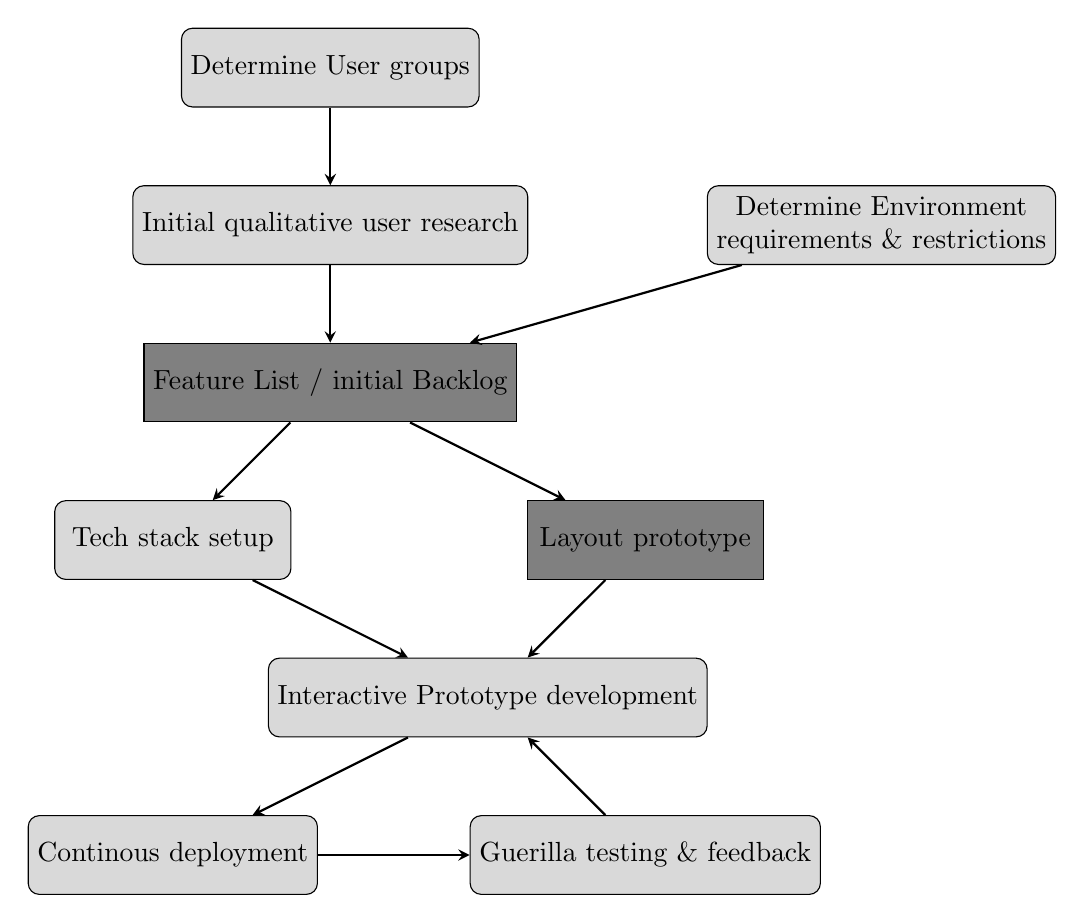
\begin{tikzpicture}[node distance=2cm]
  \tikzstyle{round} = [rectangle, rounded corners, minimum width=3cm, minimum height=1cm,text centered, draw=black, fill=gray!30]
  \tikzstyle{rect} = [rectangle, minimum width=3cm, minimum height=1cm,text centered, draw=black, fill=gray]
  \tikzstyle{arrow} = [thick,->,>=stealth]

  \node (dug) [round] {Determine User groups};
  \node (interview1) [round, below of=dug] {Initial qualitative user research};
  \node (denv) [round, right of=interview1, xshift=5cm, align=center] {Determine Environment\\requirements \& restrictions};
  \draw [arrow] (dug) -- (interview1);
  \node (bl) [rect, below of=interview1] {Feature List / initial Backlog};
  \draw [arrow] (denv) -- (bl);
  \draw [arrow] (interview1) -- (bl);
  \node (tech1) [round, below of=bl, xshift=-2cm] {Tech stack setup};
  \node (layout) [rect, right of=tech1, xshift=4cm] {Layout prototype};
  \draw [arrow] (bl) -- (tech1);
  \draw [arrow] (bl) -- (layout);
  \node (proto) [round, below of=tech1, xshift=4cm] {Interactive Prototype development};
  \draw [arrow] (tech1) -- (proto);
  \draw [arrow] (layout) -- (proto);
  \node (deploy) [round, below of=proto, xshift=-4cm] {Continous deployment};
  \draw [arrow] (proto) -- (deploy);
  \node (feedback) [round, right of=deploy, xshift=4cm] {Guerilla testing \& feedback};
  \draw [arrow] (deploy) -- (feedback);
  \draw [arrow] (feedback) -- (proto);
\end{tikzpicture}
